\begin{figure}[t]
\centering
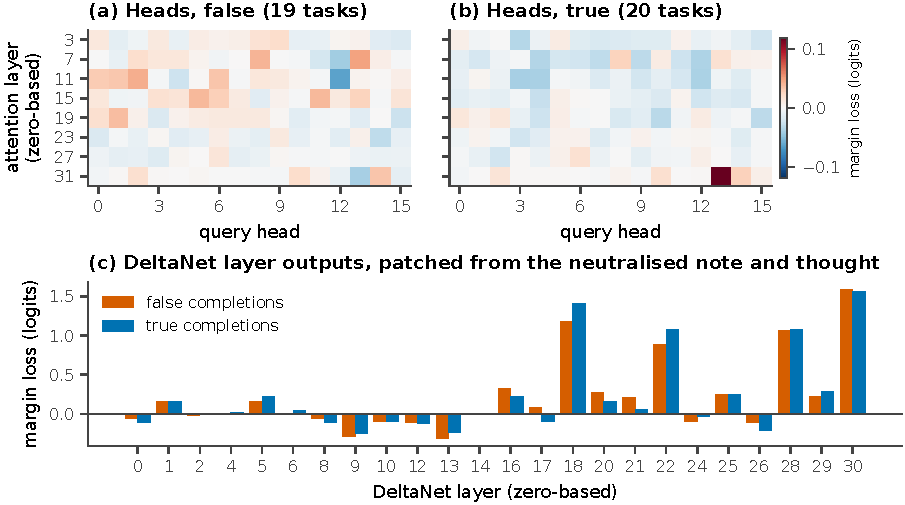
\includegraphics[width=\linewidth]{figs/moonleak.pdf}
\caption{\textbf{The written conclusion reaches the tool choice through the DeltaNet memory, for true completions as for false ones.} Teacher-forced \texttt{answer} margin lost when the note and thought are neutralised, on the strictly feasible cohort. (a, b)~Blocking the final query's attention to the note and thought, one head at a time: at most \mlHeadMaxAny{} logits (colour scale). (c)~Replacing one DeltaNet layer's output at the decision position by its value under the neutralised note and thought: \mlDeltaTopMin--\mlDeltaTopMax{} logits at layers \mlDeltaTopLayers, alike for both strata (note the ten times larger scale). Single-layer patches do not add up to the whole effect (\mlNeutralFs{} and \mlNeutralTrue{} logits). Heads and layers are screened on the same cohort: exploratory.}
\label{fig:moonleak}
\end{figure}
